%%%%%%%%%%%%%%%%%%%%%%%%%%%%%%%%%%%%%%%%%%%%%%%%%%%%%%%%
%%%%                                              %%%%%%
%%%%  Author: Peter Wilson                        %%%%%%
%%%%                                              %%%%%%
%%%%  Stabilty analysis of Mises truss                        %%%%%%
%%%%                                              %%%%%%
%%%%%%%%%%%%%%%%%%%%%%%%%%%%%%%%%%%%%%%%%%%%%%%%%%%%%%%%

\chapter[Analytical stability analysis of Mises truss]{Analytical stability\\ analysis of Mises truss}
\label{app:Analytical stability analysis of Mises truss}

An analytical stability analysis of the Mises truss system considered in chapter \ref{chap:chapter_2_2} is presented, employing the principle of virtual work via the 2nd Piola-Kirchhoff (PK2) stress measure and Green-Lagrange (GL) strain measure.

\begin{figure}[H]
	\centering
	\def\svgwidth{\columnwidth}
	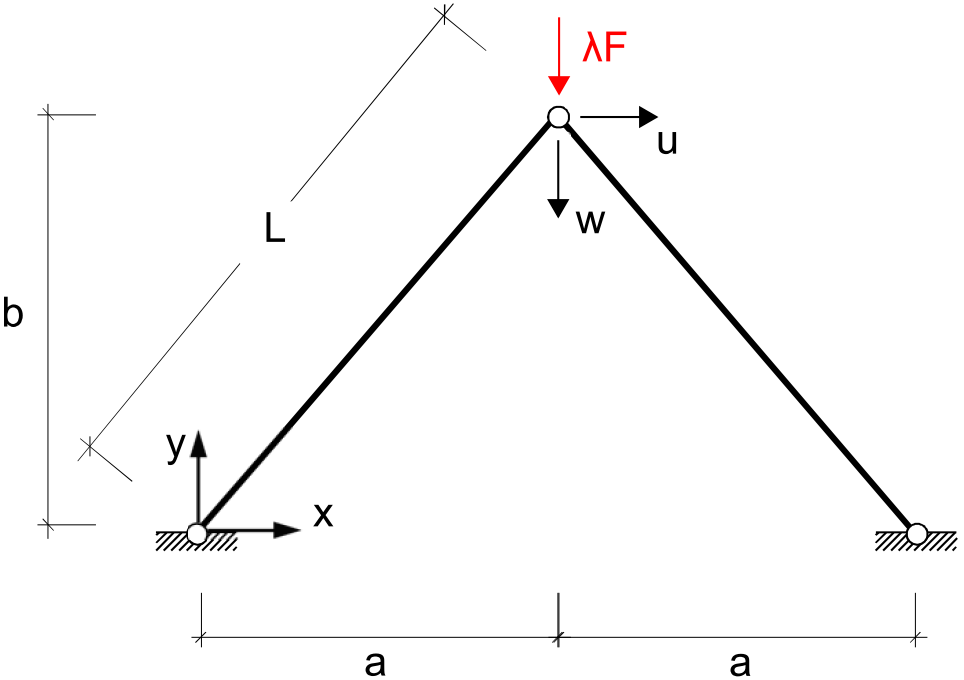
\includegraphics[width=8cm]{images/mises_truss_def.png}
	\caption{Mises truss geometry}
	\label{pic:app0}
\end{figure}

The kinematics of the system are considered first by describing the undeformed truss lengths $L$ (which are the same for both bars), deformed lengths $l$ and the Green-Lagrange strain $\epsilon_{gl}$. Truss 1 is considered first:

\begin{equation} 
L^2 = a^2 + b^2
\hspace{10mm}
l_1^2 = (a+u)^2 + (b-w)^2 = L^2 + u^2 + 2au +w^2 -2bw
\label{eqapp0_1}
\end{equation}

The Green-Lagrange strain measure for a truss is recalled and specified, as is it's first variation:

\begin{equation} 
\epsilon_{gl1} = \frac{1}{2}
\Big(\frac{l_1^2-L^2}{L^2}\Big)
=
\Big(\frac{u^2 + 2au +w^2 -2bw}{2L^2}\Big)
\hspace{10mm}
\delta\epsilon_{gl1} = 
\frac{1}{L^2}
\Big[
(u+a)\delta u
+
(w-b)\delta w
\Big]
\label{eqapp0_2}
\end{equation}

The kinematics of Truss 2 are presented:

\begin{equation} 
l_2^2 = (a-u)^2 + (b-w)^2 = L^2 + u^2 - 2au +w^2 -2bw
\label{eqapp0_2_1}
\end{equation}

\begin{equation} 
\epsilon_{gl2} = \frac{1}{2}
\Big(\frac{l_2^2-L^2}{L^2}\Big)
=
\Big(\frac{u^2 - 2au +w^2 -2bw}{2L^2}\Big)
\hspace{10mm}
\delta\epsilon_{gl1} = 
\frac{1}{L^2}
\Big[
(u-a)\delta u
+
(w-b)\delta w
\Big]
\label{eqapp0_2_2}
\end{equation}

Shifting towards stresses, the 2nd Piola-Kirchhoff stresses are linked to the Green-Lagrange strains via a linearly elastic constitutive law characterised by an axial Young's Modulus $E$.

\begin{equation} 
\sigma_{pk2} = E \epsilon_{gl}
\label{eqapp0_3}
\end{equation}

With the conjugate energy quantities defined, the virtual work expression of the system may be established, in general:

\begin{equation} 
-\delta W = \delta W_{int} - \delta W_{ext} = 0
\label{eqapp0_4}
\end{equation}

Clarifying with respect to the system considered yields:

\begin{equation} 
\delta W_{int} - \delta W_{ext} = 
\int_{V_1} \sigma_{pk2(1)} \epsilon_{gl1}
\ dV_1
+
\int_{V_2} \sigma_{pk2(2)} \epsilon_{gl2}
\ dV_2
- \lambda P \delta w = 0
\label{eqapp0_5}
\end{equation}

Combining the kinematics and constitutive relations yields a crude form of the residual vector $\mathbf{r}$:
\begin{gather} 
	\begin{aligned}
		\mathbf{r} = 
		&EAL
		\frac{1}{2L^4}
		(u^2 + 2au +w^2 -2bw)
		\Big[
		(u+a)\delta u
		+
		(w-b)\delta w
		\Big] +
		\\
		&EAL
		\frac{1}{2L^4}
		(u^2 - 2au +w^2 -2bw)
		\Big[
		(u-a)\delta u
		+
		(w-b)\delta w
		\Big] 
		- \lambda P \delta w = 0
		\label{eqapp0_6_0}
	\end{aligned}
\end{gather}

Development of the above expression, and arranging into vector form yields:

\begin{equation} 
\mathbf{r} = 
\frac{EA}{L^3}
\begin{pmatrix}
u^3+uw^2-2bwu+2a^2u \\
u^2w + w^3 - 3bw^2 - bu^2 +2b^2w - \lambda P
\end{pmatrix}
=
\mathbf{0}
\label{eqapp0_6_1}
\end{equation}

Recalling that the system tangent matrix $\mathbf{K}$ is the gradient of the system residual, as per equation \ref{eqstab01}, it can be expressed as follows:

\begin{equation} 
\mathbf{K} = 
\frac{\partial \mathbf{r}}{\partial \mathbf{u}}
=
\frac{EA}{L^3}
\begin{pmatrix}
3u^2 + w^2 - 2bw +2au +2a^2 & 2uw -2bu \\
2uw - 2bu & u^2 + 3w^2 - 6bw + 2b^2
\end{pmatrix}
\label{eqapp0_7}
\end{equation}

Key to stability analysis are the calculation of critical points which indicate the onset of instability. These points occur when the determinant of the tangent matrix vanishes, which reduces to the following expression:

\begin{equation} 
(w^2 - 2bw +2a^2)
(3w^2 -6bw +2b^2) = 0
\label{eqapp0_8}
\end{equation}

For the system considered ($a=b=EA=P=1$), the roots of the above equation are:

\begin{equation} 
w_{crit1} = 0.4226
\hspace{10mm}
w_{crit2} = 1.5774
\label{eqapp0_9}
\end{equation}

By substituting these into the system residual the corresponding critical load factors can be determined:

\begin{equation} 
\lambda_{crit1} = 0.1361
\hspace{10mm}
\lambda_{crit2} = -0.1361
\label{eqapp0_10}
\end{equation}

With the non-linear portion of the analysis complete, a linearised prebuckling analysis of the system is considered. The general eigenproblem solved in the LPB analysis is recalled from equation \ref{eqstab5}.

 \begin{equation} 
det\big[
\mathbf{K}_e +
{\lambda}
\mathbf{K}_g(\lambda_{ref})
\big]\mathbf{z} = 0
\label{eqapp0_11}
\end{equation}

The elastic matrix $\mathbf{K}_e$ is easily determined from $\mathbf{K}(\mathbf{u} = \mathbf{0})$, while the geometric stiffness matrix $\mathbf{K}_g$ for a truss is determined as follows:

 \begin{equation} 
\mathbf{K}_g = 
\frac{N}{l}
\label{eqapp0_12}
\end{equation}

$N$ is the normal force in the trusses, derived from vertical static equilibrium, and can also be expressed in terms of the applied load. Furthermore, under the LPB assumption of small displacements, the deformed and undeformed lengths are considered equivalent $l \approx L$. Thus, $\mathbf{K}_g$ can be reduced to:

 \begin{equation} 
\mathbf{K}_g = 
\frac{-\lambda P}{b}
\begin{pmatrix}
1 & 0 \\
0 & 1
\end{pmatrix}
\label{eqapp0_13}
\end{equation}

The general LPB eigensystem, focussed on critical load factors only, can be assembled:

 \begin{equation} 
 det
\begin{pmatrix}
\frac{EA}{L^3} 2a^2 - \frac{\lambda P}{b} & 0 \\
0 &  \frac{EA}{L^3} 2b^2 - \frac{\lambda P}{b}
\end{pmatrix}
= 0
\label{eqapp0_14}
\end{equation}

For the system considered ($a=b=EA=P=1$), the LPB critical load factors coalesce and are calculated to be:

\begin{equation} 
\lambda_{lpb\ crit1} = 
\lambda_{lpb\ crit2} = 0.7071
\label{eqapp0_15}
\end{equation}